\documentclass[10pt,twocolumn,letterpaper]{article}

\usepackage{cvpr}
\usepackage{times}
\usepackage{epsfig}
\usepackage{graphicx, color, xcolor}
\usepackage{amsmath}
\usepackage{amssymb}
\usepackage{bm}
\usepackage[utf8]{inputenc}
\usepackage{fancyhdr}
\usepackage{graphicx}
\usepackage[brazil]{babel}
\usepackage{lipsum}
\usepackage{float}
\setlength{\headheight}{1.5cm}

\fancypagestyle{plain}
\lhead{
\includegraphics[width=5cm,height=2cm]{logoFT.png}}
\rhead{
\includegraphics[width=5cm,height=2cm]{logoUnB.png}}

\renewcommand{\headrulewidth}{1pt}%
}

% Changing the caption and 'References' names to Portuguese.
\addto\captionsenglish{
  \renewcommand{\figurename}{Figura}
  \renewcommand{\tablename}{Tabela}
  \renewcommand{\refname}{Referências bibliográficas}
}

% to-do: Using fontenc with T1 font encoding allows \hyphenation to take words with accents
% as arguments. However, fontenc with T1 mess up with words containing 'ã' in all \subsection{}
% commands.
% If someone knows how to fix it, tell me!
%
%\usepackage[T1]{fontenc}

% Put the words not correctly hyphenated down here. Words with accents must
% be manually hyphenated in the text itself using the '\-' separator. See the examples
% throughout this template.
\hyphenation{co-e-ren-te u-sa-do de-li-mi-ta-do-res a-cer-ca va-lo-res cor-res-pon-den-te re-fe-ren-ci-a-das co-lu-na co-lu-nas em-bo-ra u-ti-li-da-de pro-ce-di-men-to ex-pe-ri-men-to fi-gu-ras}

% If you comment hyperref and then uncomment it, you should delete
% egpaper.aux before re-running latex.  (Or just hit 'q' on the first latex
% run, let it finish, and you should be clear).
\usepackage[breaklinks=true,bookmarks=true]{hyperref}

\cvprfinalcopy % *** Uncomment this line for the final submission

%\def\cvprPaperID{****} % *** Enter the CVPR Paper ID here
%\def\httilde{\mbox{\tt\raisebox{-.5ex}{\symbol{126}}}}

% Pages are numbered in submission mode, and unnumbered in camera-ready
% \ifcvprfinal\pagestyle{empty}\fi
%\setcounter{page}{1}


\begin{document}
%%%%%%%%% TITLE
\title{Experimento 2: Imperfeições AC dos Amplificadores Operacionais}

\author{Aluno 1\\
% To save space, use either the email address or home page, not both
{\tt\small 231012826@aluno.unb.br}\\
% Matrícula do primeiro autor
{\tt\small 231012826}\\
% Turma
{\tt\small Turma T02}
}

\maketitle
%\thispagestyle{empty}

%%%%%%%%% OBJETIVO

\begin{objetivo}
% Resumo com não mais de 250 palavras.
O objetivo deste experimento é compreender as diferentes imperfeições presentes nos amplificadores operacionais reais, distinguindo-as do modelo ideal estudado em aulas teóricas. Busca-se, ainda, verificar o funcionamento prático de circuitos com amplificadores operacionais, utilizando o modelo LM741, de modo a analisar suas limitações em corrente contínua (DC) e em corrente alternada (AC). Dessa forma, pretende-se relacionar os conceitos teóricos às características observadas experimentalmente, destacando o impacto dessas imperfeições no desempenho do circuito.


\end{objetivo}

%%%%%%%%% BODY TEXT
\section{Introdução}

Entre as principais imperfeições em corrente contínua (DC) dos amplificadores operacionais destacam-se a tensão de offset de entrada, as correntes de polarização de entrada e a tensão de saturação de saída. Tais efeitos influenciam diretamente a precisão do circuito, podendo introduzir erros sistemáticos em medições e no ganho estático.

No domínio em corrente alternada (AC), o desempenho dos amplificadores operacionais é limitado pela largura de banda finita, pelo produto ganho-banda passante (GBW), pela taxa de variação máxima da tensão de saída (\textit{slew rate}) e pela resposta em frequência não ideal. Esses fatores determinam a faixa útil de operação do dispositivo em altas frequências e restringem sua capacidade de amplificar sinais rápidos ou de alta amplitude.

O presente experimento busca caracterizar algumas dessas imperfeições, em especial aquelas relacionadas ao comportamento em AC. Para tanto, analisam-se diferentes configurações de amplificadores não-inversores, variando-se o ganho e verificando como o aumento deste impacta a frequência de corte e, consequentemente, o produto ganho-banda passante.

\section{Fundamentação Teórica}

O modelo ideal de um amplificador operacional considera:
\begin{enumerate}
    \item Ganho de malha aberta infinito;
    \item Impedância de entrada infinita (corrente de entrada nula);
    \item Impedância de saída nula;
    \item Resposta em frequência ilimitada;
    \item Ausência de ruído e imperfeições.
\end{enumerate}

Na prática, entretanto, essas condições não se verificam. As imperfeições em DC incluem:

\begin{itemize}
    \item \textbf{Tensão de offset de entrada} ($V_{OS}$): pequena diferença de tensão necessária entre as entradas para que a saída seja nula.
    \item \textbf{Correntes de polarização} ($I_B$): correntes que fluem pelas entradas do op-amp, devidas à polarização dos transistores internos.
    \item \textbf{Corrente de offset} ($I_{OS}$): diferença entre as correntes de polarização das duas entradas.
    \item \textbf{Saturação da saída}: o sinal de saída não consegue ultrapassar valores próximos às tensões de alimentação, ficando limitado a uma faixa menor que $V_{CC}$.
\end{itemize}

As imperfeições em AC relacionam-se principalmente à resposta em frequência:

\begin{itemize}
    \item \textbf{Ganho em malha aberta dependente da frequência}: o ganho $A_{OL}(f)$ decai a partir de uma determinada frequência de pólo dominante.
    \item \textbf{Produto ganho-banda (GBW)}: define a frequência em que o ganho de malha fechada cai para a unidade. Para qualquer configuração não inversora, vale aproximadamente:
    \[
    f_c \approx \frac{GBW}{A_{CL}},
    \]
    onde $A_{CL}$ é o ganho de malha fechada e $f_c$ a frequência de corte.
    \item \textbf{Slew rate (SR)}: taxa máxima de variação da tensão de saída, que limita a resposta a sinais senoidais de alta frequência ou grande amplitude.
\end{itemize}

No caso do experimento realizado, o interesse está em observar como a redução da banda passante acompanha o aumento do ganho em configurações não inversoras. Assim, demonstra-se experimentalmente que, apesar das diferenças entre modelos ideais e reais, o produto $A_{CL} \cdot f_c$ tende a permanecer aproximadamente constante e próximo ao GBW especificado para o amplificador operacional utilizado (no caso, o LM741).


%-------------------------------------------------------------------------

%-------------------------------------------------------------------------


%-------------------------------------------------------------------------
\newpage
\section{Simulações}

\subsection{Buffer}

Primeiro o circuito é montado com $R_1=\infty$ e $R_2=0$, fazendo da configuração não inversora um circuito Buffer (ou seguidor de tensão).

A saída deve ter amplitude de 1.26V, mas como o ganho é unitário, a entrada também deve ter amplitude de 1.26V.

\begin{figure}[h]
\caption{Circuito não inversor (buffer)}
\begin{center}
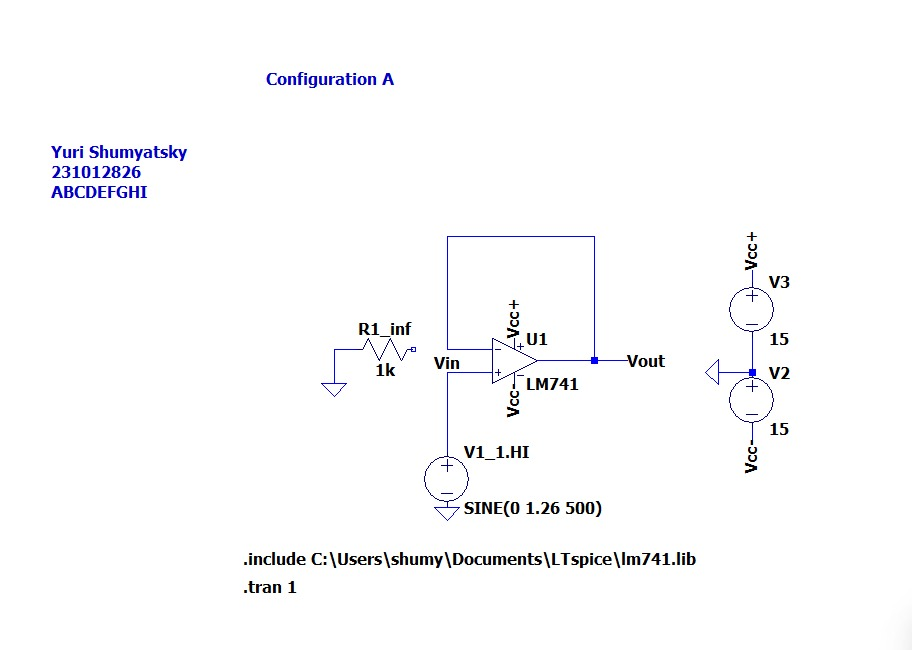
\includegraphics[scale=0.25]{figuras/fig1}
\end{center}
\end{figure}

Segue o plot das tensões de entrada e saída.

\begin{figure}[h]
\caption{Entrada e saída circuito buffer}
\begin{center}
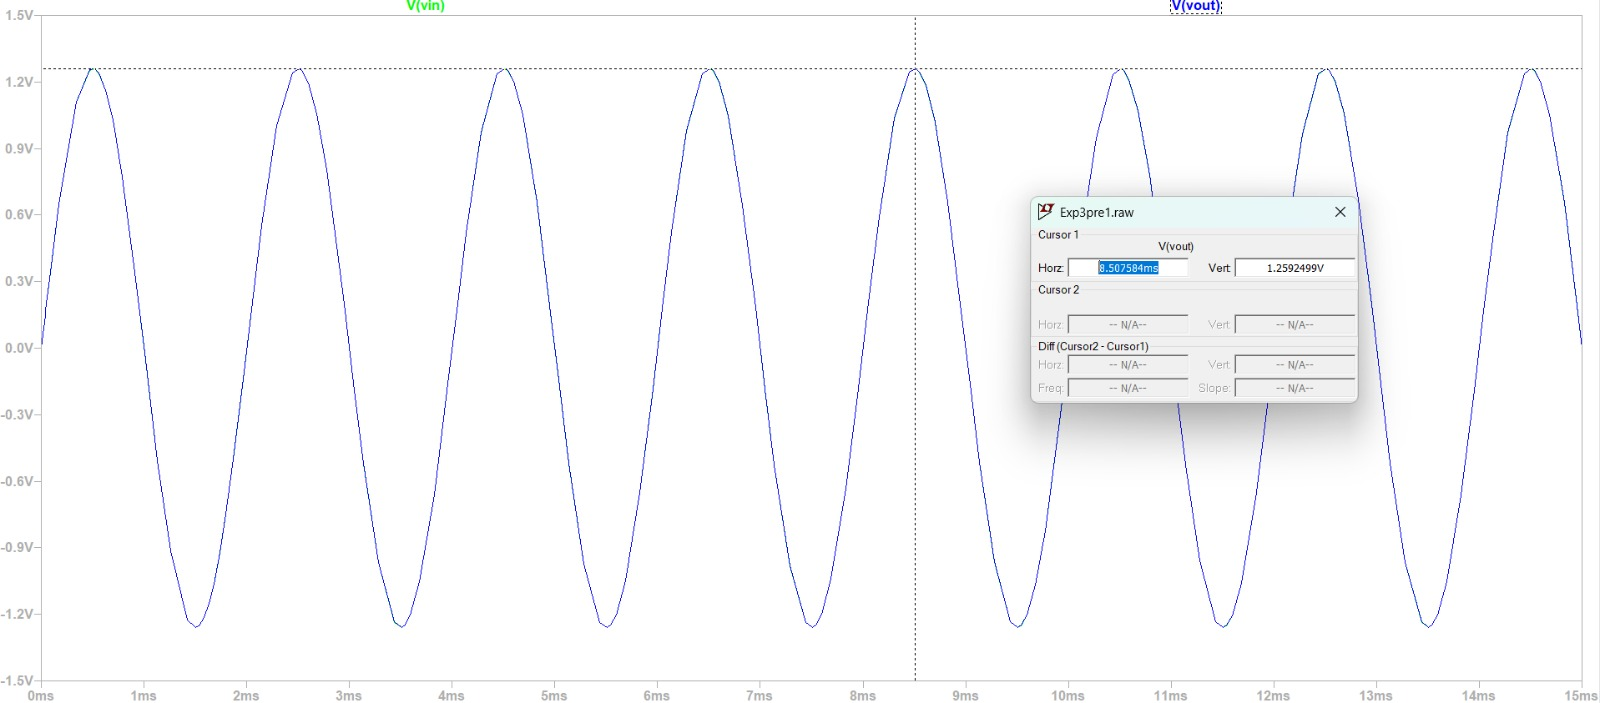
\includegraphics[scale=0.15]{figuras/fig2}
\end{center}
\end{figure}

Para encontrar a frequência de corte, foi utilizada uma análise AC para encontrar a frequência em que a amplitude cai para $(0.71)(1.26V)$.	Isso é feito ao verificar que deve ser subtraído  $20log(\sqrt{2})$ da amplitude em dB, o que equivale a subtrair 3dB pois a tensão é constante.

\begin{figure}[h]
\caption{Análise da frequência de corte}
\begin{center}
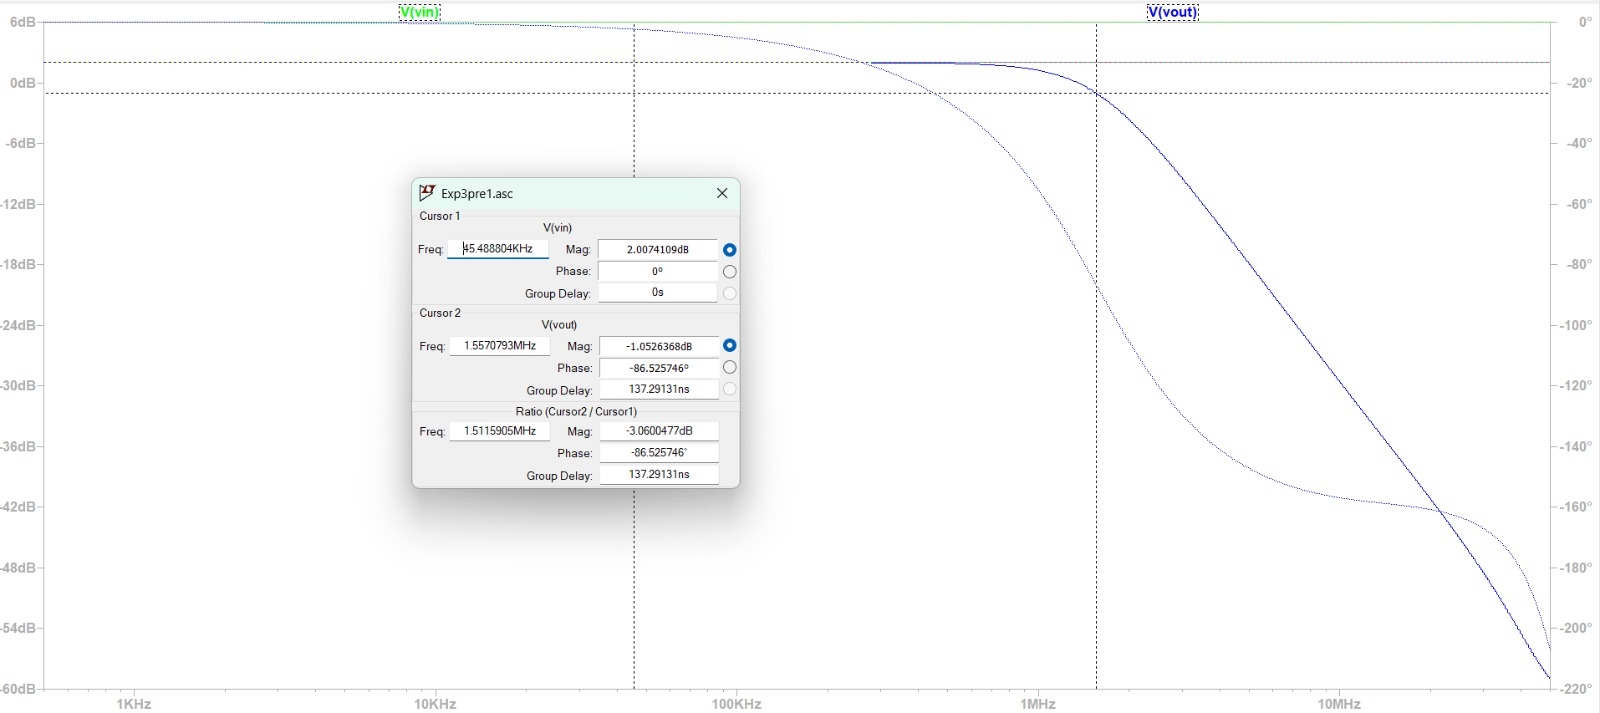
\includegraphics[scale=0.15]{figuras/fig3}
\end{center}
\end{figure}

Como pode ser observado, a $f_c$ encontrada é de 1.557MHz.

Em seguida, é plotado o ganho do circuito em seu bode plot.

\begin{figure}[h]
\caption{Plot do ganho do circuito}
\begin{center}
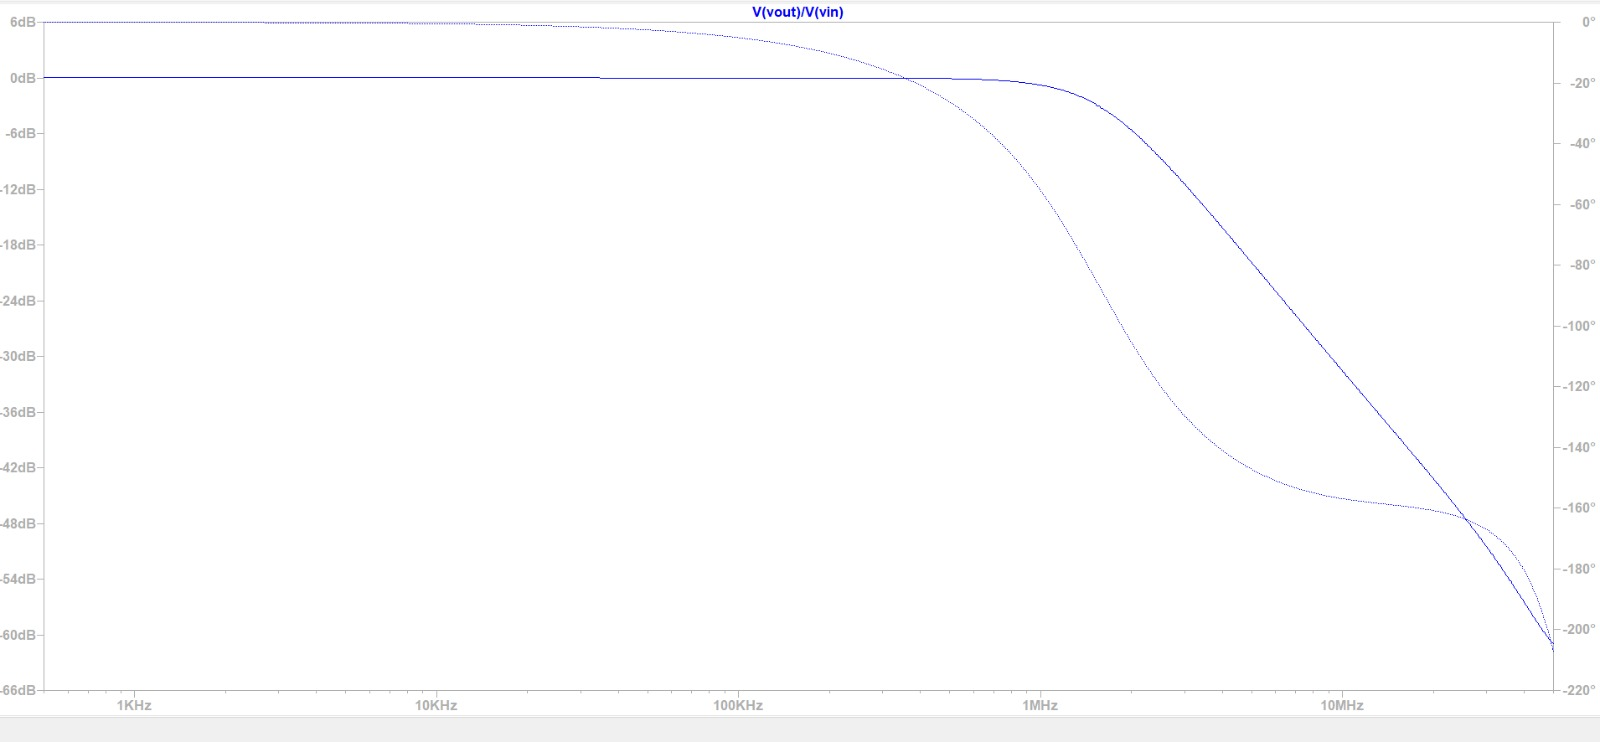
\includegraphics[scale=0.15]{figuras/fig4}
\end{center}
\end{figure}

O produto ganho $\times$ banda passante do ampop nesse circuito é $A\cdot f_c$, sendo $A$ o ganho em frequências baixas (menores que $f_c$). Como nesse circuito $A=1$ e $f_c=1.557MHz$, o produto tem valor de $1.557\cdot10^6$, como pode ser observado no seguinte gráfico.

\begin{figure}[h]
\caption{GBW}
\begin{center}
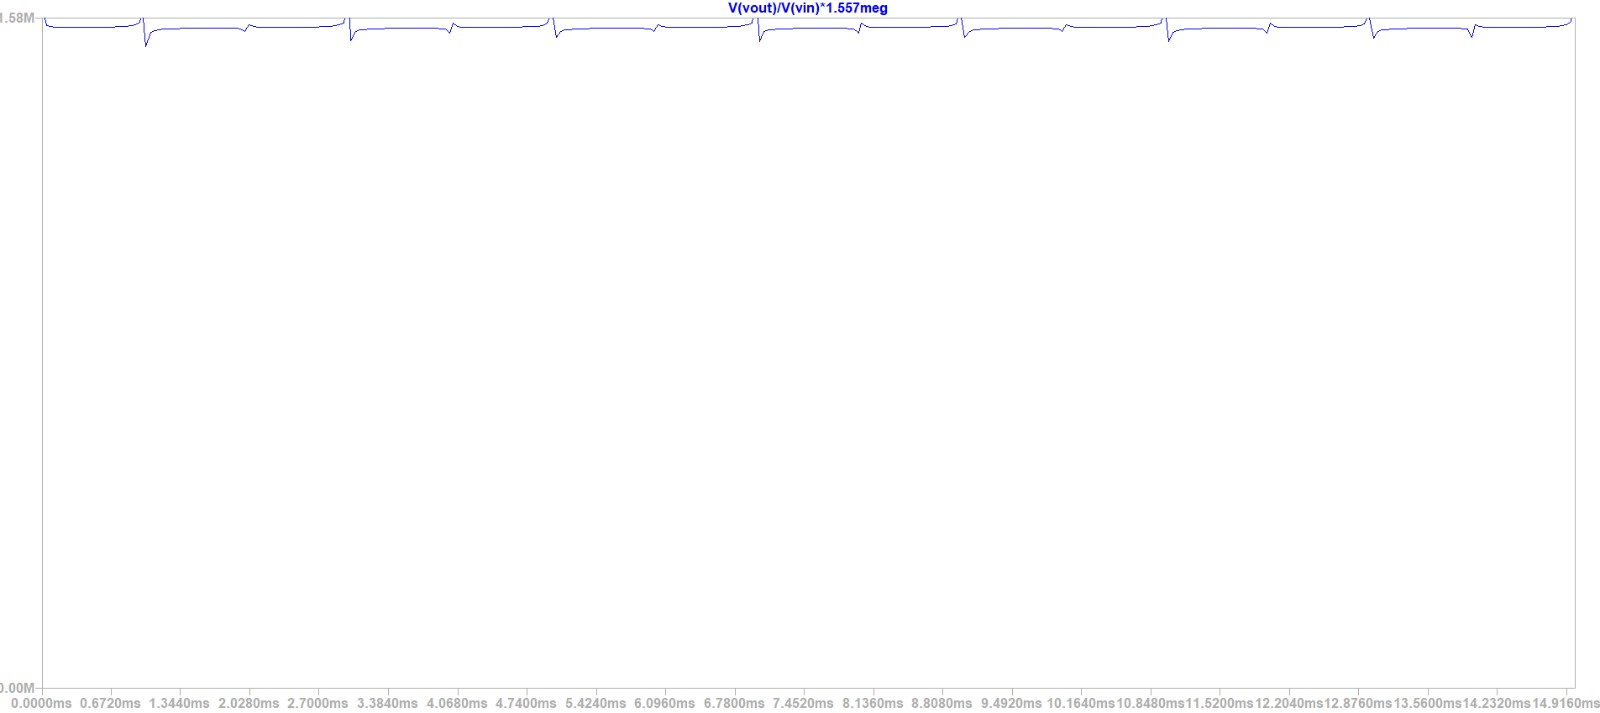
\includegraphics[scale=0.15]{figuras/fig5}
\end{center}
\end{figure}

\newpage
\subsection{Não inversor com ganho baixo}

O circuito agora é montado com $R_1=1k\Omega$ e $R_2=13k\Omega$. O ganho do circuito é 14, então para que a tensão de saída possua amplitude de $1.26V$ a tensão de entrada deve ter amplitude de $0.09V$.

\begin{figure}[h]
\caption{Circuito com ganho baixo}
\begin{center}
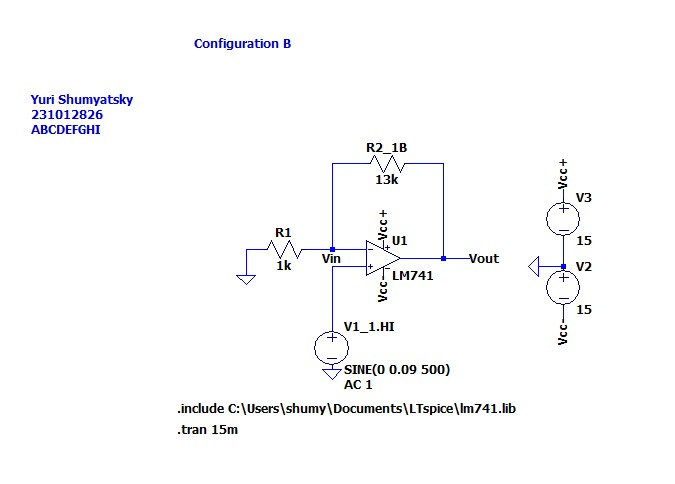
\includegraphics[scale=0.25]{figuras/fig6}
\end{center}
\end{figure}

Seguem as tensões de entrada e saída.

\begin{figure}[h]
\caption{Entrada e saída circuito com ganho baixo}
\begin{center}
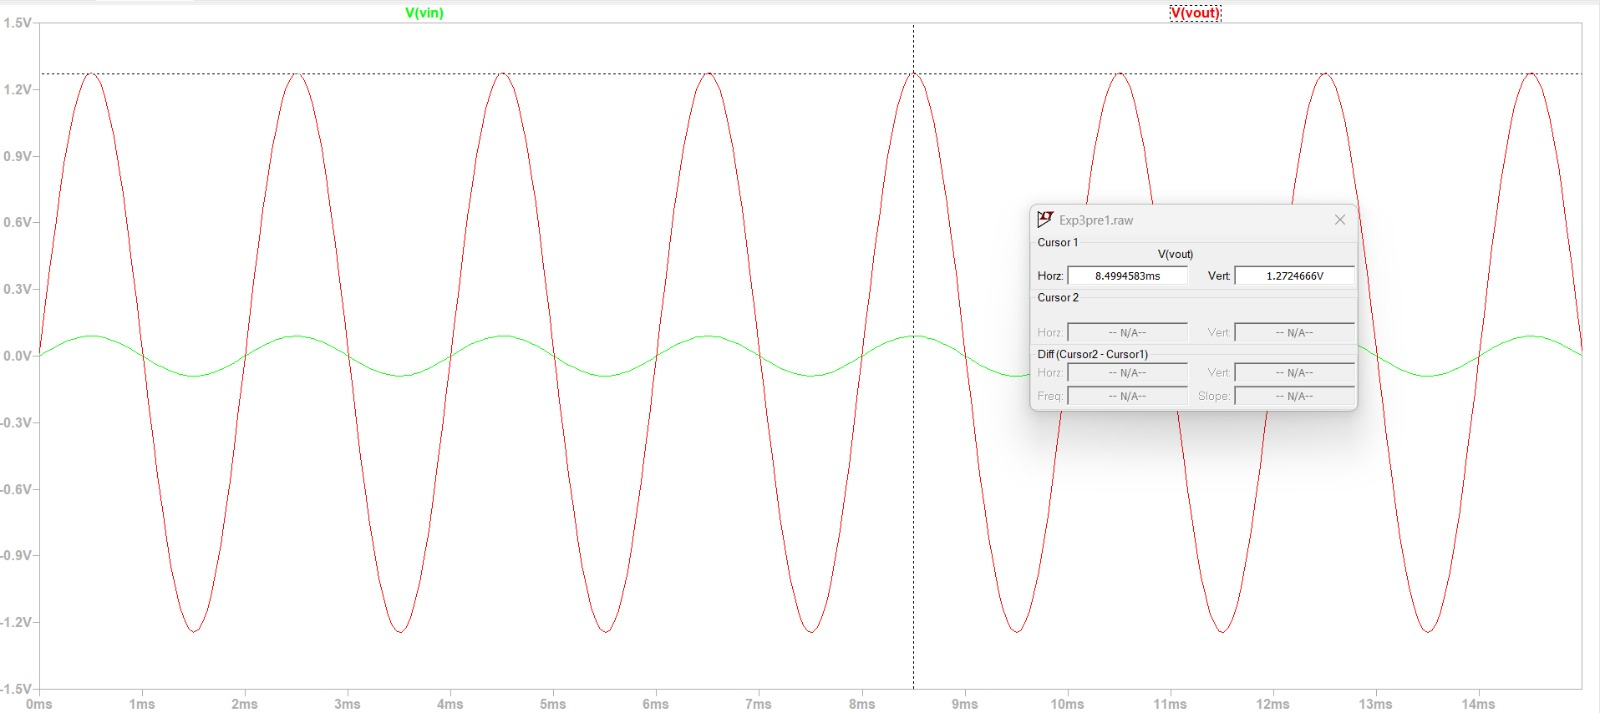
\includegraphics[scale=0.15]{figuras/fig7}
\end{center}
\end{figure}


O procedimento para encontrar a frequência de corte é análogo, tendo como resultado $f_c= 1.285$MHz

\begin{figure}[h]
\caption{Análise frequência de corte (circuito 2)}
\begin{center}
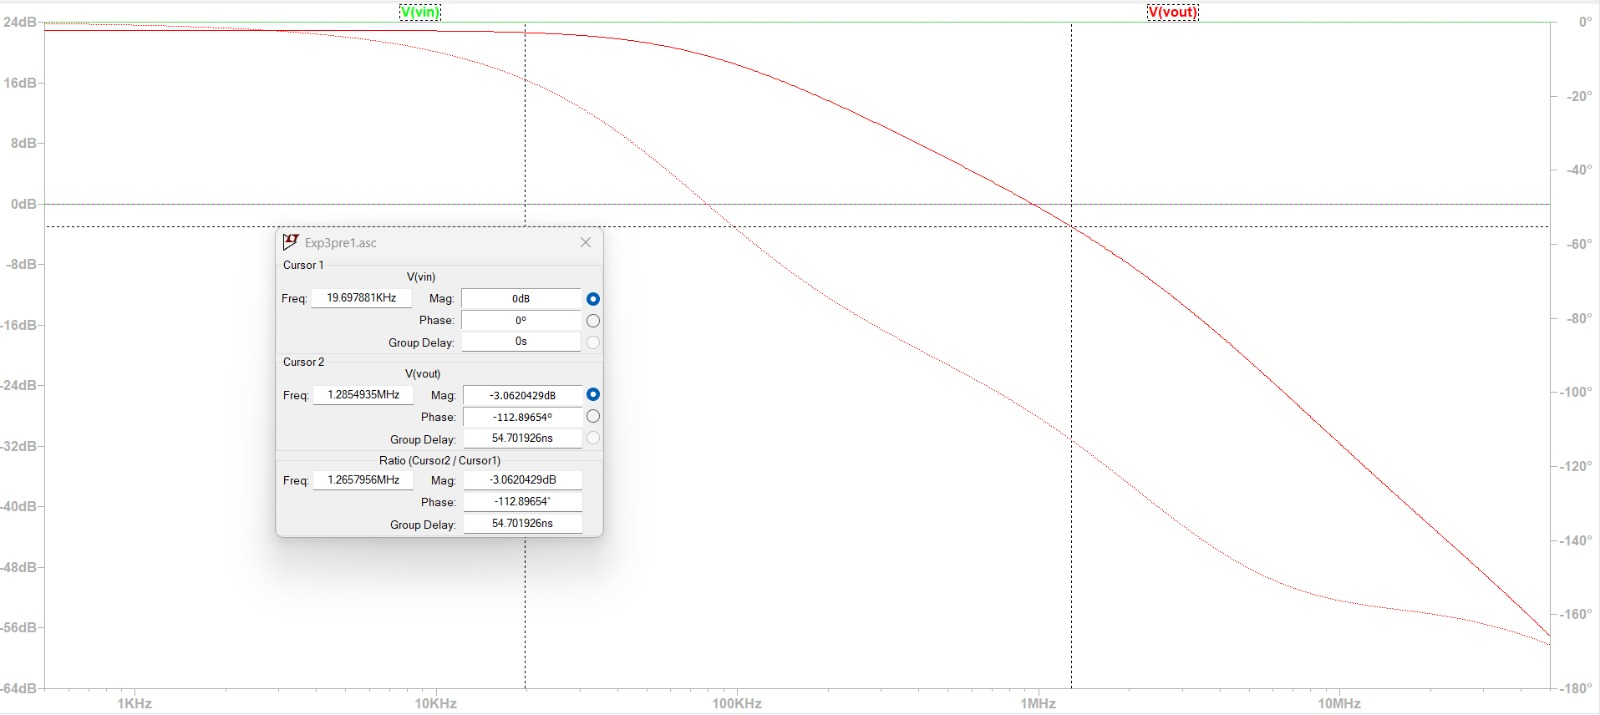
\includegraphics[scale=0.15]{figuras/fig8}
\end{center}
\end{figure}

\newpage
Segue o bode plot do ganho do circuito.

\begin{figure}[h]
\caption{Bode plot ganho (circuito 2)}
\begin{center}
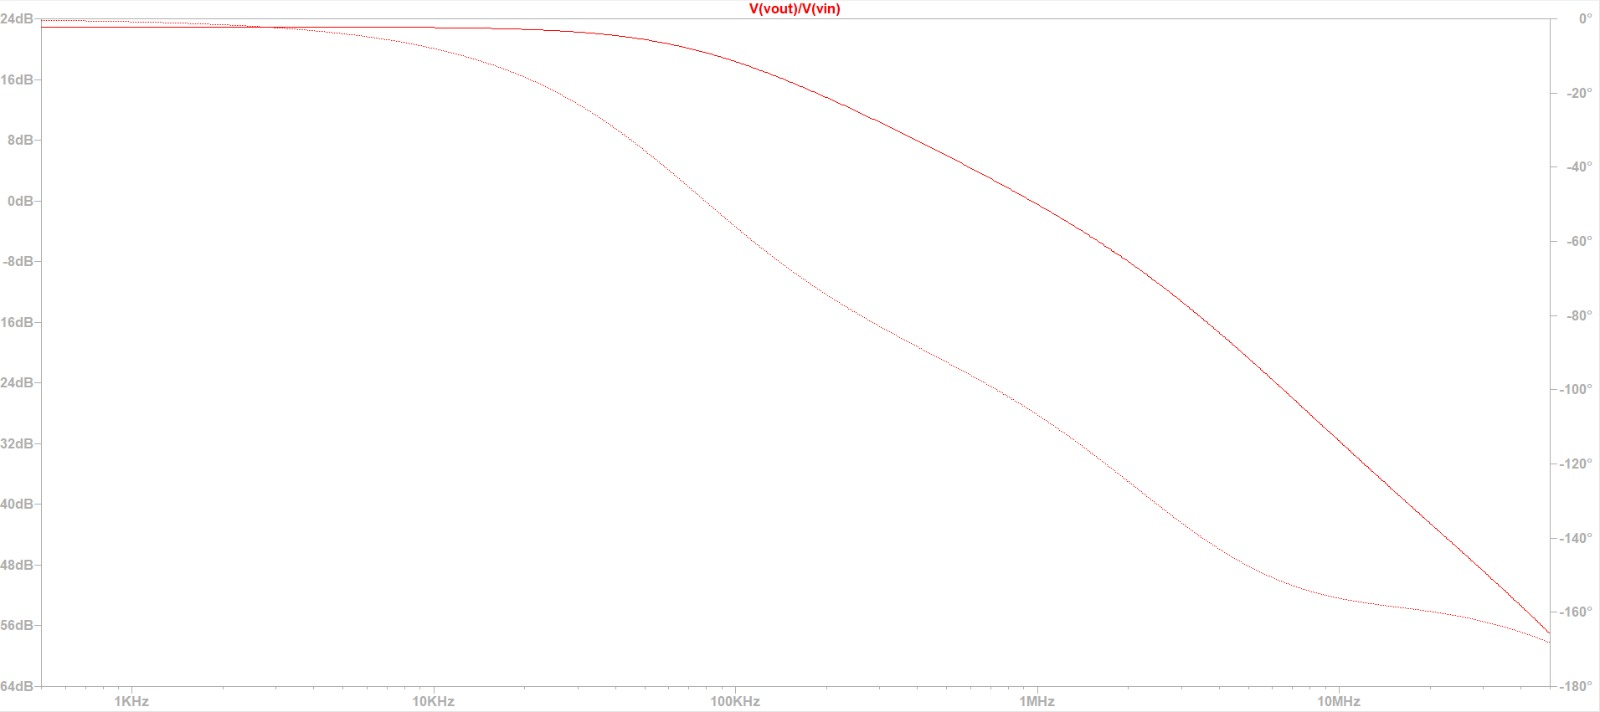
\includegraphics[scale=0.15]{figuras/fig9}
\end{center}
\end{figure}

O produto ganho $\times$ banda passante do ampop nesse circuito é $A\cdot f_c$, sendo portanto $GBW = 14\cdot1.285\cdot10^6=17.99\cdot10^6$

\begin{figure}[h]
\caption{GBW (circuito 2)}
\begin{center}
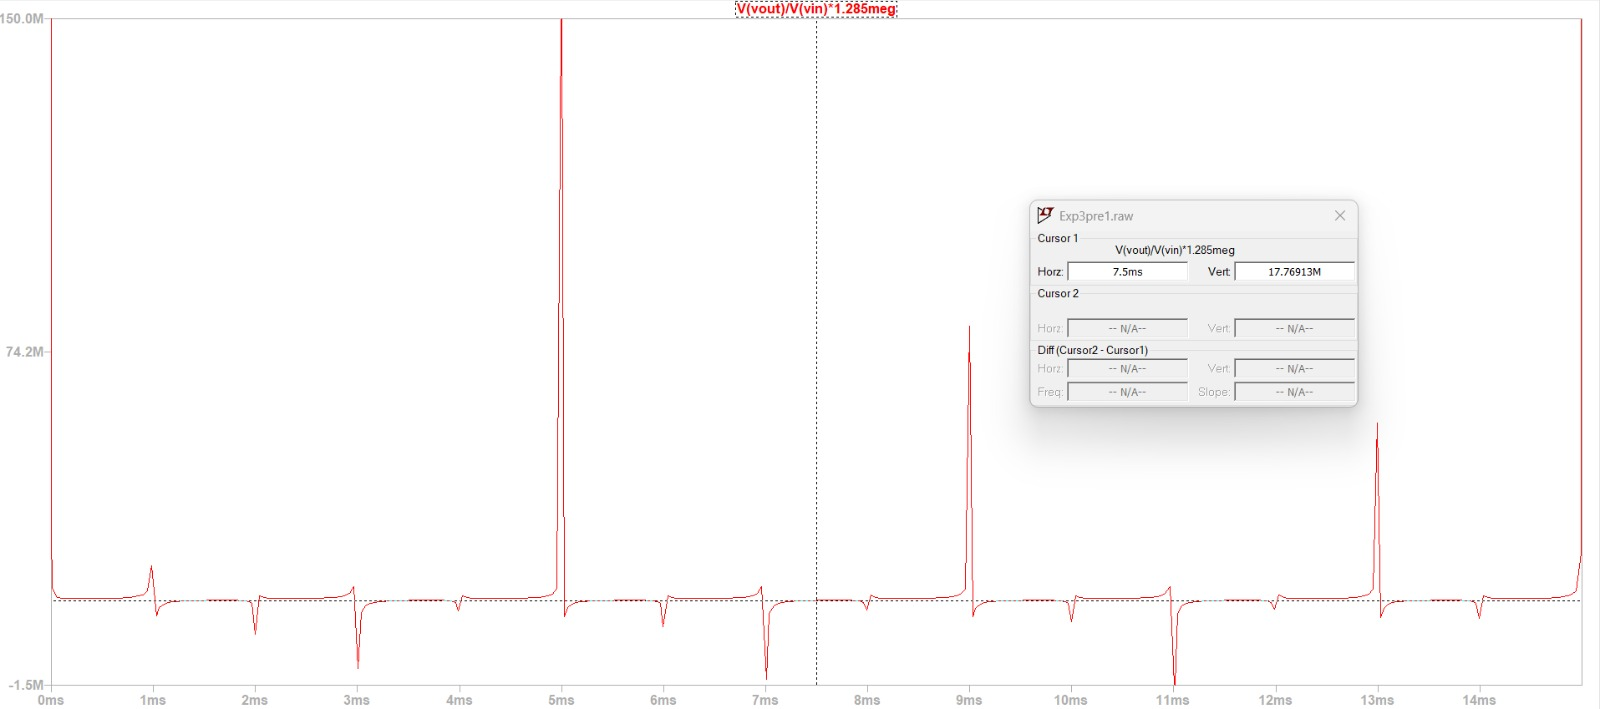
\includegraphics[scale=0.15]{figuras/fig10}
\end{center}
\end{figure}

\subsection{Circuito não inversor de ganho alto}

O circuito agora é remontado com $R_1=1k\Omega$ e $R_2=101k\Omega$. Assim, o ganho é de 102, o que faz com que para que a saída possua amplitude de $1.26V$, a entrada deve ter $0.012V$.

\begin{figure}[h]
\caption{Circuito 3}
\begin{center}
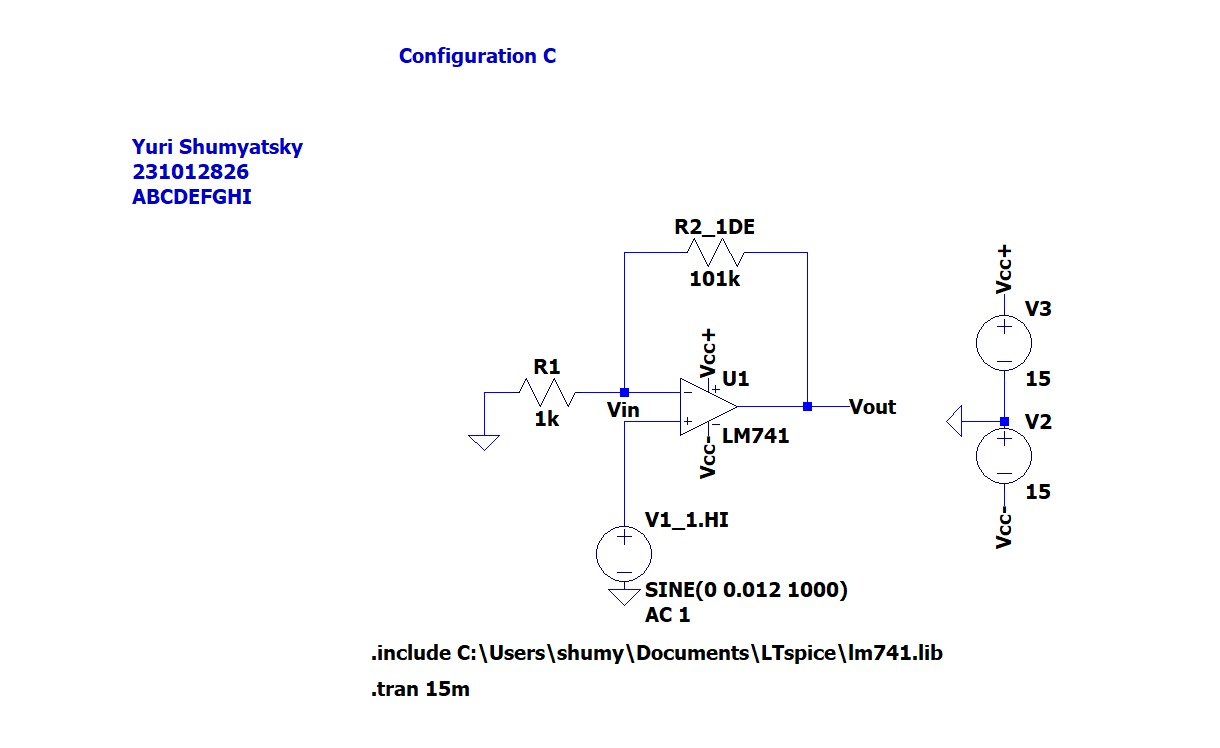
\includegraphics[scale=0.2]{figuras/fig11}
\end{center}
\end{figure}

Seguem a entrada e saída plotadas.

\begin{figure}[h]
\caption{Tensões de entrada e saída (circuito 3)}
\begin{center}
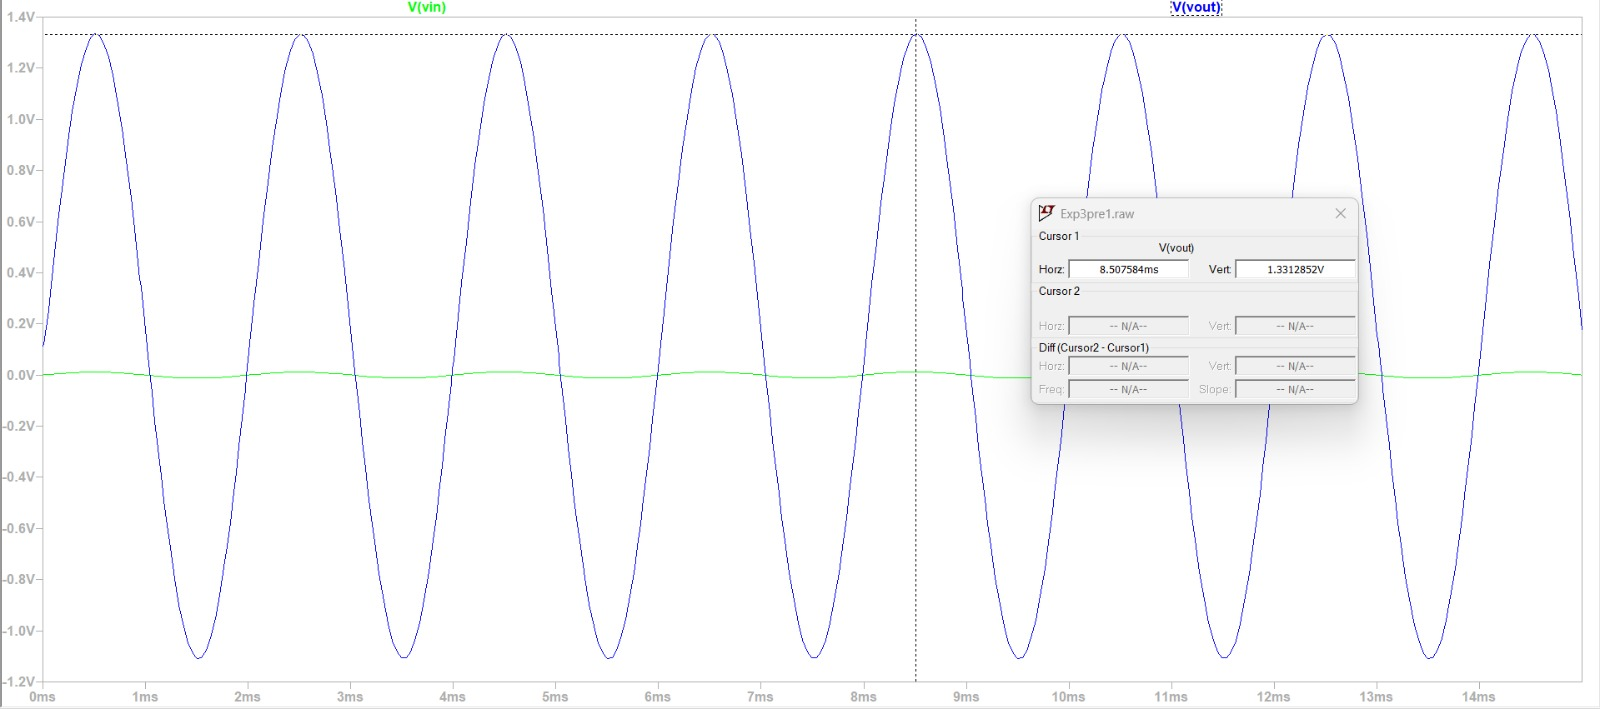
\includegraphics[scale=0.15]{figuras/fig12}
\end{center}
\end{figure}

Encontrar a frequência de corte novamente é análogo, resultando em $f_c=1.269$MHz.

\begin{figure}[h]
\caption{Análise frequência de corte (circuito 3)}
\begin{center}
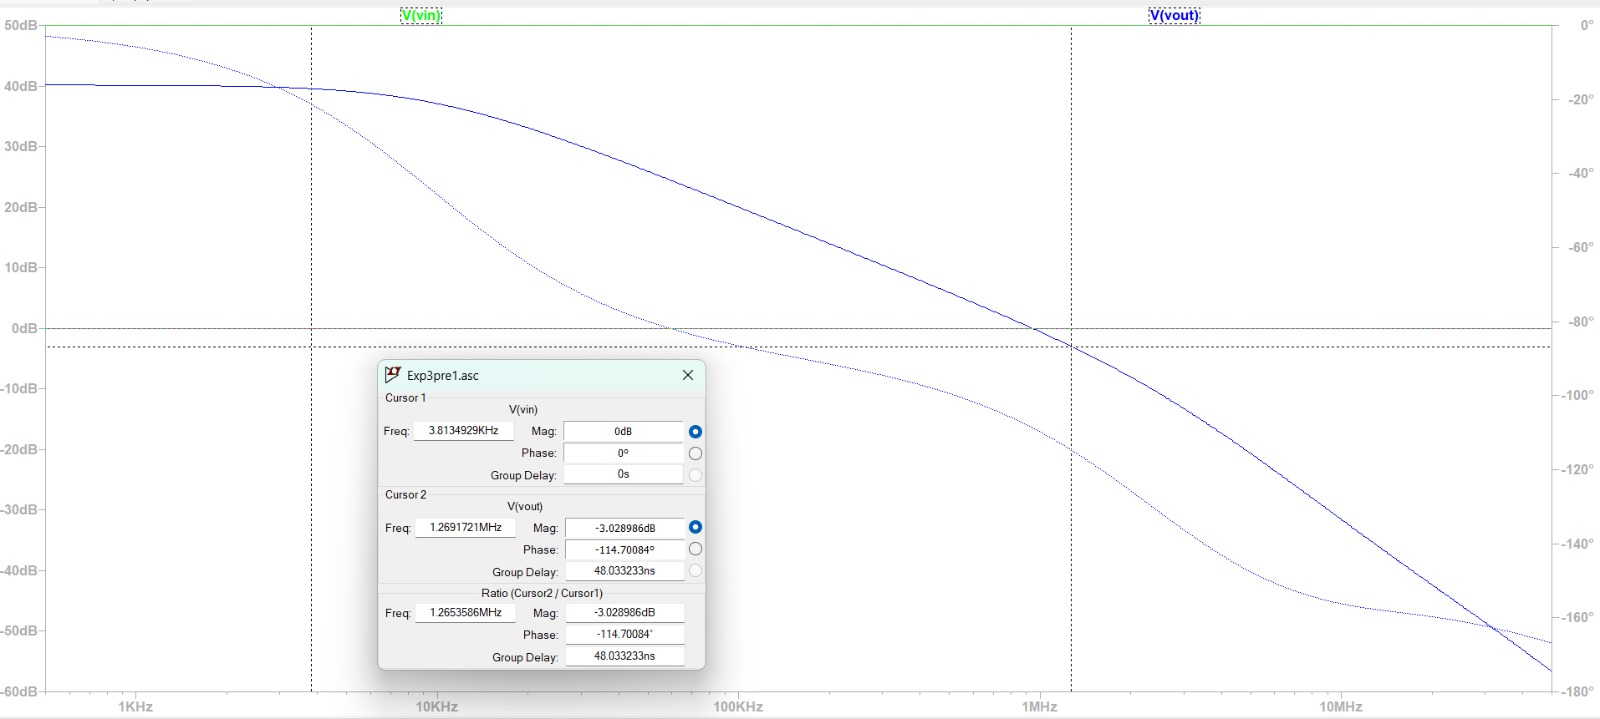
\includegraphics[scale=0.15]{figuras/fig13}
\end{center}
\end{figure}

A figura 14 é o bode plot do ganho do circuito.

\begin{figure}[h]
\caption{Bode plot do ganho (circuito 3)}
\begin{center}
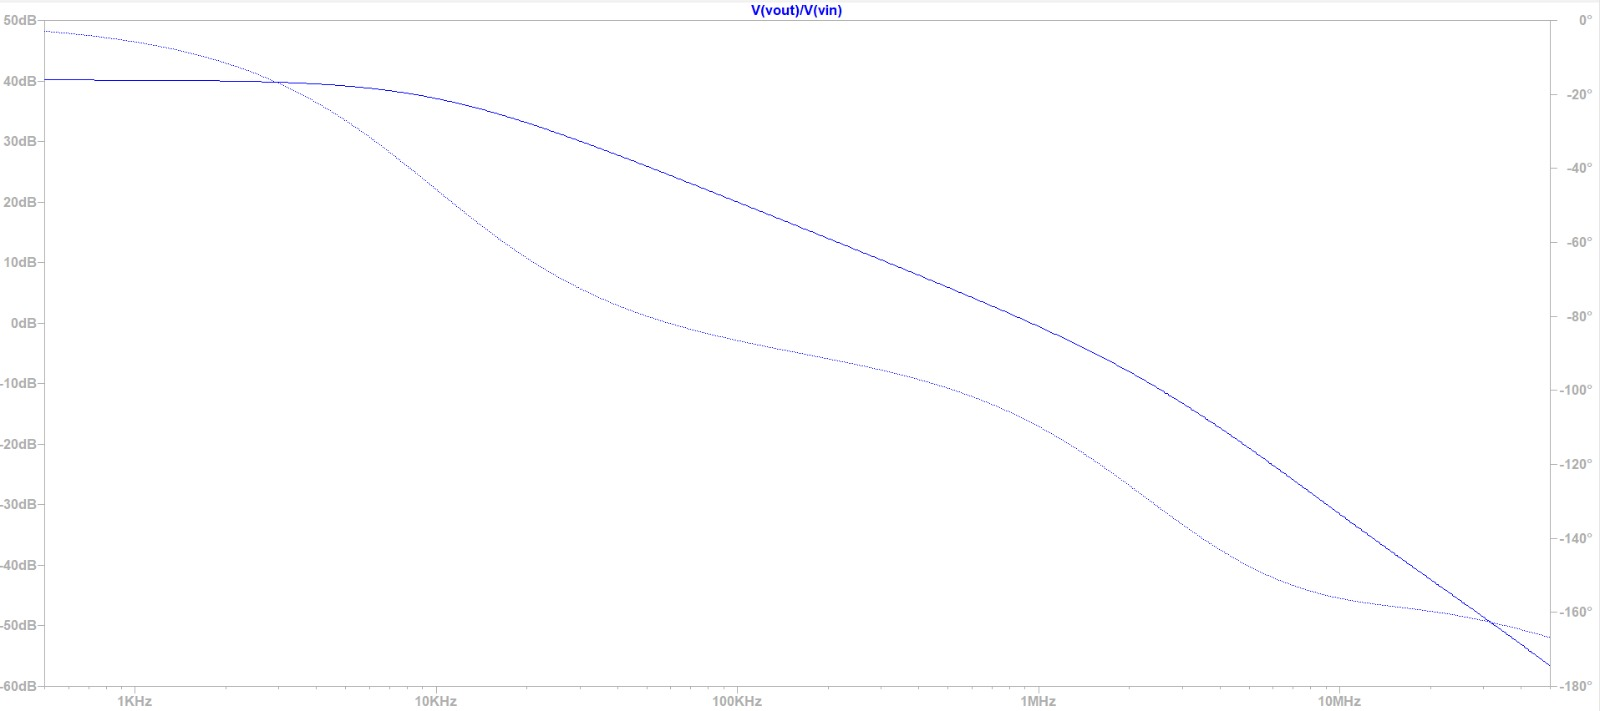
\includegraphics[scale=0.15]{figuras/fig14}
\end{center}
\end{figure}


O produto ganho $\times$ banda passante do ampop nesse circuito continua sendo $A\cdot f_c$, sendo portanto $GBW = 102\cdot1.269\cdot10^6=129.4\cdot10^6$ O analisado bate com o razoável, porém com certa margem de erro. 

\begin{figure}[h]
\caption{GBW (circuito 3)}
\begin{center}
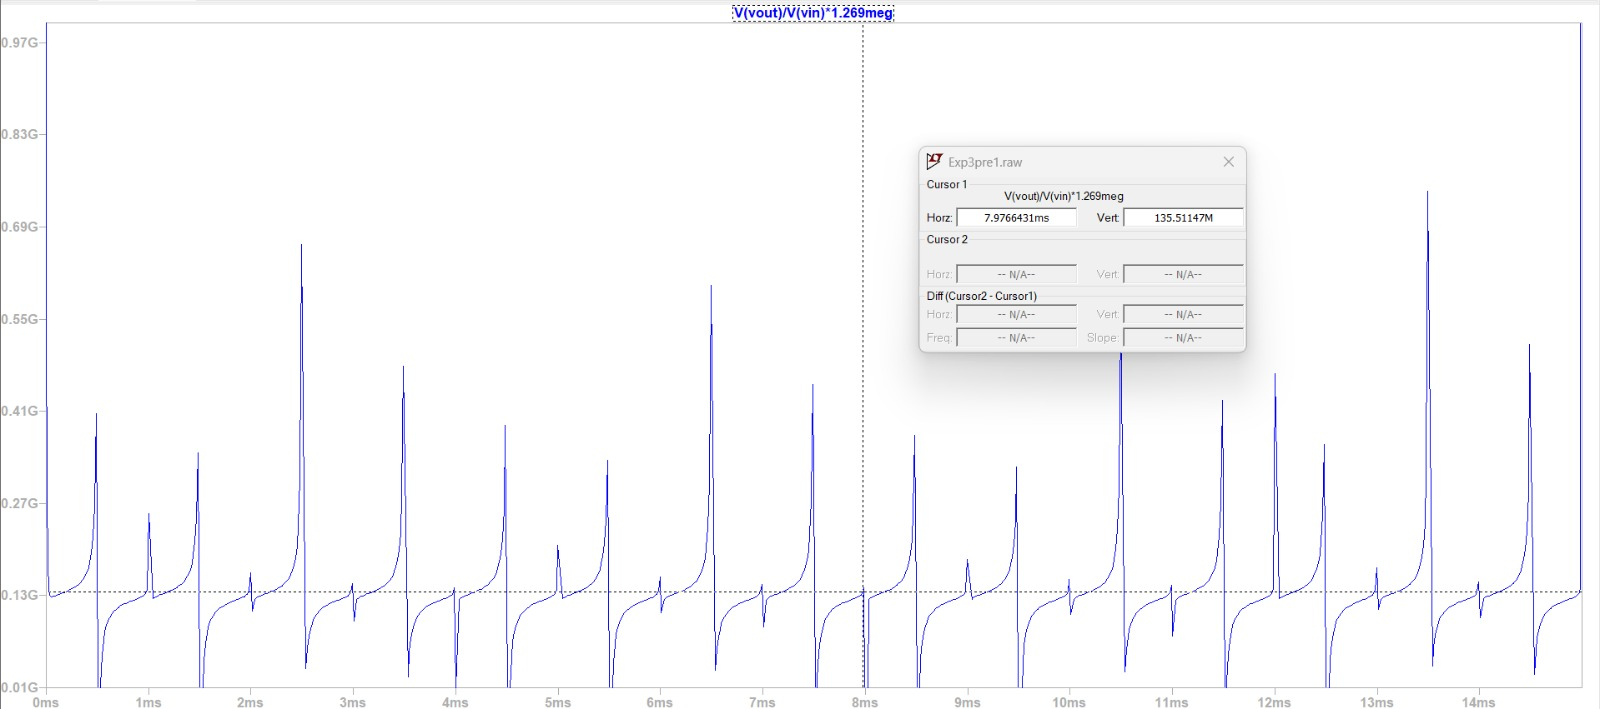
\includegraphics[scale=0.15]{figuras/fig15}
\end{center}
\end{figure}

%-------------------------------------------------------------------------


{\small
\bibliography{egbib}
\bibliographystyle{ieee_fullname}
}

\begin{itemize}
\item Razavi, B. Fundamentos de Microeletrônica, 2\textordfeminine Edição, LTC, 2014.
\end{itemize}

\end{document}
